\section{Introduction to Stochastic Differential Equations}
We have ahready seen a very simple example of SDE in ep. (4) and (5) where $x(t)=x_{0}+\mu t+\sigma B(t)$ or $d x=\mu d t+\sigma d B(t)$. This was also easy to integrate numerically. Usually an ODE has the form
(25) $\frac{d x}{d t}=f(x, t)$

Con we write an SDE in this usual form? Let's try. We get from

$$ \frac{d x}{d t}=\mu+\sigma \dot{B}(t) $$ 

What is $\dot{B}$ ? Actually it does not exist because we have seen that Brownian motion is nowhere differentiable. However, $\Delta B=B(t+\Delta t)-B(t)$ is well defined, so mathemoticions prefer the notation $d x=\mu d t+\sigma d B$. However, we can give a meaning to the "prued nototion" $\dot{B}$. We finst discretize and then take the limit as $\Delta t \rightarrow 0$; so we define for a finite $\Delta t \quad \xi_{\Delta, i}=\frac{\Delta B_{i}}{\Delta t}, \Delta B_{i} \equiv B\left(t_{i}+\Delta t\right)-B\left(t_{i}\right)$. As we know, $\Delta B_{i}$ does not depend on $t_{i}$, but this notation is useful in the following. Of course, $\left\langle\xi_{\Delta, i}\right\rangle=0$. In order to understand what $\left\langle\xi_{\Delta, i} \xi_{\Delta, j}\right\rangle$ is, let's take a test function $g(t)$ and calculate at $g_{i} \equiv g\left(t_{i}\right)$ the following

$$
\begin{gathered} 
\sum_{j} g_{j}\left\langle\xi_{\Delta, i} \xi_{\Delta, j}\right\rangle \Delta t=\sum_{j} g_{j}\left\langle\frac{\Delta B_{i}}{\Delta t} \frac{\Delta B_{j}}{\Delta t}\right\rangle \Delta t=\sum_{j} g_{j} \frac{\left\langle\Delta B_{i} \Delta B_{j}\right\rangle}{\Delta t}= \\ 
=\sum_{j} g_{j} \frac{\delta_{i j} \Delta t}{\Delta t}=g_{i} \quad N 3:\left\langle\Delta B_{i} \Delta B_{j}\right\rangle=\delta_{i j} \Delta t 
\end{gathered}
$$ 

If we now take the continuum limit $\Delta t \rightarrow 0$, and " $\lim _{\Delta t \rightarrow 0} \xi_{\Delta, i} \equiv \xi(t)$ " we get

$$
\int g\left(t^{\prime}\right)\left\langle\xi(t) \xi\left(t^{\prime}\right)\right\rangle d t^{\prime}=g(t)
$$ 

Which therefore means that $\left\langle\xi(t) \xi\left(t^{\prime}\right)\right\rangle=\delta\left(t-t^{\prime}\right)$ and $\langle\xi(t)\rangle=0$. This is called Gaussian white (or $\delta$-correlated) noise; with this we con then write the SDE in ef. (4) as
(26) $\begin{gathered}
\dot{x}(t)=\mu+\sigma \xi(t) \\
\langle\xi\rangle=0 \quad\left\langle\xi(t) \xi\left(t^{\prime}\right)\right\rangle=\delta\left(t-t^{\prime}\right)\end{gathered} \quad$ is equivalent to

$$
 d x=\mu d t+\sigma d B(t)
$$ 

$B(t)$ is a standard $B M \langle B\rangle=0\langle B(t) B(s)\rangle=t \wedge s$

The finst one is a mototion which physicists like the most, whereas mothematicions prefer $d x=\mu d t+d B$, you con find both in the literature.

What is a solution?
If we stort from a deterministic ey like

$$
 d x=f(x, t) d t
$$ 

there are many ways to introduce noise. We could define a stoch. process by saying that $d x=\tilde{f}(x, t, d B) d t$ where $\tilde{f}$ is a generic non-linear surooth function. However this definition does not work in general and it is very difficult to define appropriately what that exactly meons and to able to find solutions.
The approach that warks in many situations, even in higher dimensions under general assumptions is to introduce the noise (better, Brownion motion) in an additive way. This means that we con develop
a good daol of theory for SDES of the form
(27) $d x=\mu(x, t) d t+\sigma d B(t) \quad(\sigma>0)$
where $\mu$ is a suroth function of $x, t$. This ey. can be also justified on physical grounds as we will see in the following (if $x(t)$ is the position of a large particle in a fluid, $\operatorname{cdB}$ con represent the effect of all other suall fluid particles at temperature $T$, and $\sigma=\sigma(T)$, which continuously kick the longe one. All kicks produce the erratic movement of the big suspended perticle).
Eq. (27) is colled Longevin equation with additive noise.
However, even simple equations such as this one

$$
 d x=-\mu x d t+\sigma d B
$$ 

con hide pitfolls. For instence, $\langle d x\rangle=-\mu\langle x\rangle d t$, so $\frac{d\langle x\rangle}{d t}=-\mu\langle x\rangle$ hence $\langle x(t)\rangle=x_{0} e^{-\mu t}$. But what about fluctuations?

We need to colculate $\left\langle x^{2}\right\rangle$. Let's proceed naively with ordinary colculus: $\quad \frac{d x^{2}}{d t}=2 x \frac{d x}{d t}$, so $2 x d x=-2 \mu x^{2} d t+\sigma 2 x d s$ and $d\left\langle x^{2}\right\rangle=2\langle x d x\rangle=-2 \mu\left\langle x^{2}\right\rangle d t+2 \sigma\langle x d B\rangle=-2 \mu\left\langle x^{2}\right\rangle d t$ =o?
then $\frac{d\left\langle x^{2}\right\rangle}{d t}=-2 \mu\left\langle x^{2}\right\rangle \Rightarrow\left\langle x^{2}\right\rangle=x_{0}^{2} e^{-2 \mu t}$. But then

$$
 \sqrt{\left\langle x^{2}\right\rangle}=x_{0} e^{-\mu t}=\langle x\rangle \Rightarrow \operatorname{Var}[x(t)]=0!
$$ 

So there are no fluctuations even if we add the noise! Either ordinary colculus comot be used or $\langle x d B\rangle \neq 0$ This is a consequence of the non-differentiability of $B$.

We con consider SDEs even more general SDEs thon q.(2T) driven by Brownion restion
(28) $d x=\mu(x, t) d t+\sigma(x, t) d B$

This is an SDE with multiplicative noise because $\sigma$ is a function of the state $x$. Eq. (28) needs extra core!

If we have a (strong) solution $x(t)$ of $\%$. (28) then we con write
(28b) $x(t)=x(0)+\int_{0}^{t} \mu(x(s), s) d s+\int_{0}^{t} \sigma(x(s), s) d B(s)$
A strong solution is some functional $F(t, B(s), s \leq t)$ of the Brownion motion $B(t)$. This becomes the selution of the consesponding $O D E$ as $\sigma=0$.

Warning:
What is the meaning of $\int_{0}^{t} \sigma(x(s), s) d B(s)$ ? Con this be understaod as an ordinary integral? No.

Let's take a veiy simple example. If the process is simply $(\mu=0$ and $\sigma=B)$:

$$
 d x=B(t) d B(t)
$$ 

the olution is $\quad X(t)=\int_{0}^{t} B(s) d B(s)$
So we nairely expect $E[x(t)]=0$

If we use ordinary calculus then

$$
 x(t)=\frac{B(t)^{2}}{2}
$$ 

but then $\mathbb{E}[x(t)]=\frac{t}{2} \neq 0$. What's going on here?
Again, becouse Brownion motion is very irregular, it gives rise to problems where interpreting solutions or eps.

Before showing what the nature of the problem is, we have to prove an ireportant property of the Brownion m.

LEMMA: The Brownian motion has finite quadratic variation Let's fix $t>0$, take the interval $[0, t]$ and partitions $\mathcal{P}_{n}$ of the interval $\left\{t_{0}=0<t_{1}<t_{2} \cdots<t_{n}=t\right\}$ such that $\left|D_{n}\right| \equiv \operatorname{mot}_{i}\left|t_{i}-t_{i-1}\right| \left|P_{n}\right| \rightarrow 0$ as $n \rightarrow \infty$. Then
(29)

$$
 \operatorname{ms-lim}_{\substack{n \rightarrow \infty \\\left|\theta_{m}\right| \rightarrow 0}} \sum_{0}^{n-1} \underbrace{\left[B\left(t_{i+1}\right)-B\left(t_{i}\right)\right]^{2}}_{\text{quadratic variation}}=t
$$ 

Reminder: $\underset{n \rightarrow \infty}{m s-\lim } x_{n}=x$ means $\lim _{n \rightarrow 
\infty}\left\langle\left(x_{n}-x\right)^{2}\right\rangle=0$ this is the mean square limit and we say that $x_{m}$ converges $t b$ in the mean square.

Proof: Let's define $Q_{n} \equiv \sum_{0}^{m-1}\left[B\left(t_{i+1}\right)-B\left(t_{i}\right)\right]^{2}$ and take

$$
 Q_{n}-t=\sum_{i}\left\{\left[B\left(t_{i+1}\right)-B\left(t_{i}\right)\right]^{2}-\left(t_{i+1}-t_{i}\right)\right\} .
$$ 

Hence we have to evaluate os $n \rightarrow \infty \quad\left(B\left(t_{i}\right) \equiv B_{i}\right)$
(29b)

$$
 \mathbb{E}\left[
\left(Q_{m}-t\right)^{2}\right]=\sum_{0}^{m-1} i \sum_{j}^{m-1} \mathbb{E}\left[\left\{\left(B_{i+1}-B_{j}\right)^{2}-\left(t_{i+1}-t_{i}\right)\right\}\left\{\left(B_{j+1}-B_{j}\right)^{2}-\left(t_{j+1}-t_{j}\right)\right\}\right]=
$$ 

For $i \neq j$

$$
 \begin{aligned}
& \mathbb{E}\left[\left\{\left(B_{i+1}-B_{i}\right)^{2}-\left(t_{i+1}-t_{i}\right)\right\}\left\{\left(B_{j+1}-B_{j}\right)^{2}-\left(t_{j+1}-t_{j}\right)\right\}\right]=\leftarrow \text{ indo } \\
&= \mathbb{E}\left[\left\{\left(B_{i+1}-B_{i}\right)^{2}-\left(t_{i+1}-t_{i}\right)\right\}\right] \mathbb{E}\left[\left\{\left(B_{j+1}-B_{j}\right)^{2}-\left(t_{j+1}-t_{j}\right)\right\}\right]=0 \\
& \mathbb{E}\left[
\left(B_{i+1}-B_{i}\right)^{2}\right]=t_{i+1}-t_{i}
\end{aligned}
$$ 

Therefore ep. (29b) becomes

$$
 \begin{aligned}
& \mathbb{E}\left[
\left(Q_{m}-t\right)^{2}\right]=\sum_{0}^{m-1} \mathbb{E}\left[\left\{\left(B_{i+1}-B_{i}\right)^{2}-\left(t_{i+1}-t_{i}\right)\right\}^{2}\right]=
 \\
& =\sum_{i}\left\{\mathbb{E}\left[
\left(B_{i+1}-B_{i}\right)^{4}\right]-2 \mathbb{E}\left[
\left(B_{i+1}-B_{i}\right)^{2}\right]\left(t_{i+1}-t_{i}\right)+\left(t_{i+1}-t_{1}\right)^{2}\right\}=
 \\
& \text{ the } 4^{\text{re }} \text{ moment of } N\left(0, t_{i+1}-t_{i}\right) \text{ is } 3\left(t_{i+1}-t_{i}\right)^{2} \\
& =\sum_{i}\left\{3\left(t_{i+1}-t_{i}\right)^{2}-2\left(t_{i+1}-t_{i}\right)^{2}+\left(t_{i+1}-t_{i}\right)^{2}\right\}=
 \\
& =2 \sum_{i}\left(t_{i+1}-t_{i}\right)^{2} \leq 2 \sum_{i}\left(t_{i+1}-t_{i}\right) \operatorname{mot}_{m}\left(t_{i+1}-t_{i}\right)=2\left|\operatorname{O}_{m}\right| t \rightarrow 0
\end{aligned}
$$ 

One con show that the convergence is even stronger, it is alwast sure: $\lim _{n} Q_{n}=t$. $\partial t$ is remarkable that, although $Q_{n}$ is rondom for any finite $n$, its limit is not!

This lemma portly justifies the heuristic idea that $|d B| \simeq \sqrt{d t}$
(30) which we will use many times in the future.

If we interpet $x(t)=\int_{0}^{t} B(s) d B(s)$ as the limit of Riemann sums as in the ordinary definition of integrals, we have to chiscretize it and then take the limit. The fellowing theorem will show the nature of the "poslem".

\section*{Theorem.}
Let's take the interval $[0, t](t>0)$ and partitions $\mathcal{P}_{n}$ of the interval $\left\{t_{0}=0<t_{1}<t_{2} \cdots<t_{n}=t\right\}$ such that $\left|D_{n}\right| \equiv \operatorname{mot}_{i}\left|t_{i}-t_{i-1}\right| \left|\mathbb{P}_{n}\right| \rightarrow 0$ as $n \rightarrow \infty$. Also fix $\lambda \in \mathbb{R}, 0 \leq \lambda \leq 1$ and define

$$
 X_{n} \equiv \sum_{0}^{n-1} B\left(\lambda t_{i+1}+(1-\lambda) t_{i}\right)\left[B\left(t_{i+1}\right)-B\left(t_{i}\right)\right]
$$ 

then

\begin{equation*}
\operatorname{lims-lim}_{\substack{n \rightarrow \infty \\\left|\theta_{m}\right| \rightarrow 0}} x_{m}=\frac{[B(t)]^{2}}{2}+\left(\lambda-\frac{1}{2}\right) t \tag{31}
\end{equation*}


\begin{center}
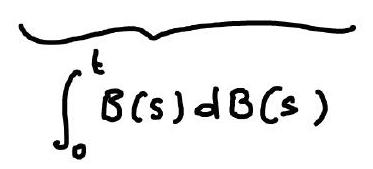
\includegraphics[width=0.5\textwidth]{2025_10_17_a59e220b8a74630d2381g-07}
\end{center}

\section*{COMMENTS:}
We reginize $x_{n}$ as the Riemonn sum conesponding to $x(t)$ where we tok an arbitrary intermediate point in $\left[t_{i}, t_{i+1}\right]$. In ordinary calculus the integral does not depend on the location of the intermediate point, however in the stochastic integral there is an unavoidable dependence on which point we chaose. This is one of the most important feotures of the stochostic calculus with Brownion motion.
proof:
We introduce a more compact notation: $B_{i}^{\lambda} \equiv B\left(\lambda t_{i+1}+(1-\lambda) t_{i}\right) B
\left(t_{i}\right) \equiv B_{i}$. Then $x_{n}=\sum_{0} i B_{i}^{\lambda}\left(B_{i+1}-B_{i}\right)$.
We use now the identity (with B.m. everything is easier with squares or squared differences:
$B_{i}^{\lambda}\left(B_{i+1}-B_{i}\right)=\left(B_{i}^{\lambda}-B_{i}+B_{i}\right)\left(B_{i+1}-B_{i}^{\lambda}+B_{i}^{\lambda}-B_{i}\right)=$

$$
 \begin{aligned}
& =\left(B_{i}^{\lambda}-B_{i}\right)\left(B_{i+1}-B_{i}^{\lambda}\right)+\left(B_{i}^{\lambda}-B_{i}\right)^{2}+B_{i}\left(B_{i+1}-B_{i}^{\lambda}\right)+B_{i}\left(B_{i}^{\lambda}-B_{i}\right) \\
& =\left(B_{i}^{\lambda}-B_{i}\right)\left(B_{i+1}-B_{i}^{\lambda}\right)+\left(B_{i}^{\lambda}-B_{i}\right)^{2}+B_{i} B_{i+1}-B_{i}^{2} \\
& A_{s} B_{i} B_{i+1}=-\frac{1}{2}\left(B_{i+1}-B_{i}\right)^{2}+\frac{1}{2} B_{i+1}^{2}+\frac{1}{2} B_{i}^{2} \\
& =\underbrace{\left(B_{i}^{\lambda}-B_{i}\right)\left(B_{i+1}-B_{i}^{\lambda}\right)}_{(\text{D})}+\underbrace{\left(B_{i}^{\lambda}-B_{i}\right)^{2}}_{(\text{C})}-\underbrace{\frac{1}{2}\left(B_{i+1}-B_{i}\right)^{2}}_{(\text{B})}+\underbrace{\frac{B_{i+1}^{2}}{2}-\frac{B_{i}^{2}}{2}}_{(A)}
\end{aligned}
$$ 

Let's colculate all the terms:
(A) $\quad \sum_{0}^{n-1} i\left(\frac{B_{i+1}^{2}}{2}-\frac{B_{i}^{2}}{2}\right)=\frac{1}{2}\left(B_{n}^{2}-B_{n-1}^{2}+B_{n-1}^{2}-B_{n-2}^{2} \cdots B_{1}^{2}-B_{0}^{2}\right)$

$$
=\frac{1}{2}\left(B_{n}^{2}-B_{0}^{2}\right)=\frac{B^{2}(t)}{2}
$$ 

(B) $-\frac{1}{2} \sum_{0}^{m-1}\left(B_{i+1}-B_{i}\right)^{2} \xrightarrow{\text { ms-linit }}-\frac{t}{2}$ (lemma)
(C) $\sum_{0}^{n-1}\left(B_{i}^{\lambda}-B_{i}\right)^{2} \xrightarrow{\text { ms-limit }} \lambda t$ (use the lemma)
(D) We have to show that the term (D) is zero in the ms-limit:

$$
 \begin{aligned}
& \mathbb{E}\left[
\left(\sum_{0}^{n-1}\left(B_{i}^{\lambda}-B_{i}\right)\left(B_{i+1}-B_{i}^{\lambda}\right)\right)^{2}\right]=\sum_{\uparrow}^{n-1} \mathbb{E}\left[
\left(B_{i}^{\lambda}-B_{i}\right)^{2}\right] \mathbb{E}\left[
\left(B_{i+1}-B_{i}^{\lambda}\right)^{2}\right]=
 \\
& \text{ indep. increments } \\
& =\sum_{0 i}^{n-1} \lambda\left(t_{i+1}-t_{i}\right) \cdot(1-\lambda)\left(t_{i+1}-t_{i}\right) \\
& \leq \lambda(1-\lambda) \operatorname{mot}_{j}\left(t_{j+1}-t_{j}\right) \sum_{0}^{n-1}\left(t_{i+1}-t_{i}\right) \leq \lambda(1-\lambda)\left|0_{n}\right| t \rightarrow 0 \text{ as } n \rightarrow \infty .
\end{aligned}
$$ 

The theorem shows that
(32) $\quad \int_{0} B(s) d B(s)=\frac{B^{2}(t)}{2}+\left(\lambda-\frac{1}{2}\right) t$
so it does depend in general on the intermediate point that we choose. The main choices are:
(I) $\quad \int_{0}^{t} B(s) d B(s)=\frac{B^{2}(t)}{2}-\frac{t}{2} \quad It \hat{a}$ integral $\lambda=0$
(S) $\quad \int_{0}^{t} B(s) \cdot d B(s)=\frac{B^{2}(t)}{2} \quad$ Stratonovich integral $\quad \lambda=\frac{1}{2}$

IMPORTANT COMMENTS:
(1) Why should we use too? Since $t$ represents time and because we do not know what value B will get in the following interval $\left[t_{i}, t_{i+1}\right]$, we prefer to select the known value in the approximetion, i.e. $B
\left(t_{i}\right)$. This is the choice in (I).

From ef. (32)

$$ 
\mathbb{E}\left[
\int_{0}^{t} B(s) d B(s)\right]=0
$$ 

So (I) has the strange property that that it does not follow ordinary colums, but it is hondy because one con show that $\mathbb{E}[B(t) d B(t)]=\mathbb{E}[B(t)] \mathbb{E}[d B(t)]=0$. In general for Itô integrals:

$$ 
E
\left[
\int \sigma d B
\right]=\int E[\sigma] E[d B]=0
$$ 

In the following we will always use the Ito prescription when considering SDEs of the form (28).

Notice that if the SDE is with additive noise (ep. (27) there is no need to introduce any intermediate prescription.
If we use a function $\sigma(x)$, instead of $B(s)$, and we define $\int_{0}^{t} \sigma(x) d B(s)$ as in $\varphi$. (28b), in general $\sigma(x)$ will depend on the $B . n . B(s)$ for $s s t$ and we do not know at time $t$ its future value at times $\tau>t$. We don't went $\sigma$ to depend on $B(t)-B(t),+>s$. All these functions $\sigma(x)$, which depend only on the information available up to five $t$ (so they are indep. of $B(t)-B(s), \forall t>s)$, are colled non-anticipating functions. We will always use these functions.
If $\sigma$ is mon-anticipoting, the 1 to stochastic integral $(\lambda=0)$ of the function $\sigma(x)$ is defined as

$$ 
\int_{0}^{t} \sigma(s) d B(s)=\lim _{n \rightarrow 
\infty} \lim ^{\text {it depends on }\{B\}}\left(\sum_{0}^{n-1} \sigma
\left(t_{i}\right)\left[B
\left(t_{i+1}\right)-B
\left(t_{i}\right)\right]\right)
$$ 

One can also show that ( $\sigma$ mon-anticipating)

$$ 
\left(\int_{0}^{t} \sigma(s) d B(s)\right)^{2}=\int_{0}^{t} d s \sigma(s)^{2}
$$ 

(See Gordiner p. 84): ms-lim $\sum_{0}^{n-1} i=\sigma_{i}\left(B_{i+1}-B_{i}\right)^{2}=\int_{0}^{t} d s \sigma(s)$
(2) The adventige with the Strotonovich choice $\left(\lambda=\frac{1}{2}\right)$ is that one con use ordinary colulus, but in this cose

$$ 
\mathbb{E}\left[
\int_{0}^{t} B(s) d B(s)\right]=\frac{t}{2}
$$ 

So the B.m. is conclated to the following times.

The dependence on the internediate point is cher even when calculating the expected value $\mathbb{E}\left[
\int_{0}^{t} B(s) d B(s)\right]$.
The discretization gives $\left(t_{0}=0, t_{m}=t\right)$

$$
 \begin{aligned}
& \mathbb{E}\left[
\sum_{0}^{n-1} B\left(t_{i}+\lambda\left(t_{i+1}-t_{i}\right)\right)\left(B\left(t_{i+1}\right)-B\left(t_{i}\right)\right)\right]=
 \\
= & \sum_{i} \underbrace{\mathbb{E}\left[B\left(t_{i}+\lambda\left(t_{i+1}-t_{i}\right)\right) B
\left(t_{i+1}\right)\right]}_{\min \left[t_{i}+\lambda\left(t_{i+1}-t_{i}\right), t_{i+1}\right]=t_{i}+\lambda\left(t_{i+1}-t_{i}\right)}-\sum_{i}\underbrace{\mathbb{E}\left[B\left(t_{i}+\lambda\left(t_{i+1}-t_{i}\right)\right) B
\left(t_{i}\right)\right]}_{\min \left[t_{i}+\lambda\left(t_{i+1}-t_{i}\right), t_{i}\right]=t_{i}}=
 \\
& =\sum_{0}^{n-1} i\left(t_{i}+\lambda\left(t_{i+1}-t_{i}\right)-t_{i}\right)=\lambda t
\end{aligned}
$$ 

Exercize: Assume thot the stochostic process $g(t)$ depends on the B.m. $B(s)$ for any $s<t$, so $g$ is non-anticipating. Show that $\mathbb{E}\left[
\left(\int_{0}^{t} g(s) d B(s)\right)^{2}\right]=E
\left[
\int_{0}^{t} g^{2}(s) d s\right]$ if we use the Ito convention.
Hint: use the discretization $\sum_{0}^{-1} i g
\left(t_{i}\right)\left(B
\left(t_{i+1}\right)-B
\left(t_{i}\right)\right)$ and, after all the colculations, take the limit $n \rightarrow \infty$.

\section*{Itô Colculus}
We have seen that the Brownion motion may lead to a change in the usual colculus. In the following we only show what are the new differentiation ules when using the Its presaription and the finding that $\Delta B \simeq \sqrt{\Delta t}$
Let's assume that $u(B(t), t)$, then

$$
 \begin{aligned}
& \Delta u=u(B(t+\Delta t), t+\Delta t)-u(B(t), t) \stackrel{\downarrow}{=} \frac{\partial u}{\partial t} \Delta t+\frac{\partial u}{\partial B} \Delta B+\frac{1}{2} \frac{\partial^{2} u}{\partial B^{2}} \Delta B^{2}+\text{ h.o.t. } \\
& =\frac{\partial u}{\partial t} \Delta t+\frac{\partial u}{\partial B} \Delta B+\frac{1}{2} \frac{\partial^{2} u}{\partial B^{2}} \Delta t+\text{ h.o.t. } \leftarrow \text{ " } \Delta B^{2}=\Delta t \text{ " } \\
& =\left(\frac{\partial u}{\partial t}+\frac{1}{2} \frac{\partial^{2} u}{\partial B^{2}}\right) \Delta t+\frac{\partial u}{\partial B} \Delta B
\end{aligned}
$$ 

this term is not present in ordinary colculus and is due to the feet that $|
\Delta B| \simeq \sqrt{\Delta t}$

The Ito differential whe is
(34)

$$
 d u=\left(\frac{\partial u}{\partial t}+\frac{1}{2} \frac{\partial^{2} u}{\partial B^{2}}\right) d t+\frac{\partial u}{\partial B} d B
$$ 

Of course, if $u$ does not depend on $t$, $d u=\frac{1}{2} \frac{\partial^{2} u}{\partial B^{2}} d t+\frac{\partial u}{\partial B} d B$.
Example: $u(B)=B^{2}$, then $d B^{2}=d t+2 B d B$. If we then integrate both sides $\int_{t_{1}}^{t_{2}} d
\left(B^{2}\right)=B^{2}
\left(t_{2}\right)-B^{2}
\left(t_{1}\right)=t_{2}-t_{1}+2 \int_{t_{1}}^{t_{2}} B(s) d B(s)$ we get

$$
 \int_{t_{1}}^{t_{2}} B(s) d B(s)=\frac{B^{2}
\left(t_{2}\right)-B^{2}
\left(t_{1}\right)}{2}-\frac{t_{2}-t_{1}}{2}
$$ 

which is in ogreement with ey. (I)

Exercize: 1) Calculate the Ito differential for $B_{t}^{n}$ and show that $d B_{t}^{n}=n B_{t}^{n-1} d B_{t}+\frac{n(n-1)}{2} B_{t}^{n-2} d t$ and $\int_{0}^{t} B^{n} d B=\frac{B_{t}^{n+1}}{n+1}-\frac{n}{2} \int_{0}^{t} B(s)^{n-1} d s$
2) By using the Ito differential of $Y(B, t)=e^{\lambda B(t)-\frac{\lambda^{2}}{2} t}$ and that $B(0)=0$, show that $Y(t)=Y(B, t)$ salves the $I$ to $S D E$

$$
 \left\{
\begin{aligned}
& d Y(t) \quad=\lambda Y(t) d B(t) \\
& Y(0) \quad=1
\end{aligned}\right.
$$ 

Show that $\langle Y(t)\rangle=1 \quad \forall t \geqslant 0$ and $P(y, t)=\frac{e^{-\frac{\left(\ln y+\frac{\lambda^{2} t}{2}\right)^{2}}{2 \lambda^{2} t}}}{\sqrt{2 \pi \lambda^{2} t} y}$. This is called log-normal distribution.

\section*{Itô's choim rule (Itô's formula)}
Suppose that $X(t)$ is a stoch. process which satisfies the SDE

$$
 d x(t)=\mu(x, t) d t+\sigma(x, t) d B(t)
$$ 

where the SDE is interpreted with the Ito prescription; then if $u(x, t) \in C_{t}^{1}, \in C_{x}^{2}$ then the stochastic process $u$ satisfies the $S D E$ :


\begin{equation*}
d u=\left(\frac{\partial u}{\partial t}+\frac{\partial u}{\partial x} \mu+\frac{1}{2} \frac{\partial^{2} u}{\partial x^{2}} \sigma^{2}\right) d t+\frac{\partial u}{\partial x} \sigma d B \tag{35}
\end{equation*}

Inoleed, we use the simple wles: $d t d B=O
\left(d t^{3 / 2}\right), d B^{2}=d t$

$$
 d u=\frac{\partial u}{\partial t} d t+\frac{\partial u}{\partial x} d x+\frac{1}{2} \frac{\partial^{2} u}{\partial x^{2}} d x^{2}+\text{ hot. }
$$ 

however $\quad d x^{2}=(\mu d t+\sigma d B)^{2}=\mu^{2} d t^{2}+2 \mu \sigma d t d B+\sigma^{2} d B^{2}=\sigma^{2} d t$
then

$$
 \begin{aligned}
& d u \quad=\frac{\partial u}{\partial t} d t+\frac{\partial u}{\partial x}(\mu d t+\sigma d B)+\frac{1}{2} \frac{\partial^{2} u}{\partial x^{2}} \sigma^{2} d t \\
& =\left(\frac{\partial u}{\partial t}+\frac{\partial u}{\partial x} \mu+\frac{1}{2} \frac{\partial^{2} u}{\partial x^{2}} \sigma^{2}\right) d t+\frac{\partial u}{\partial x} \sigma d B \text{ os in (35) }
\end{aligned}
$$ 

Exercige: 1) The stoch. proc. $x(t)$ stisfies the Ito $S D E$ (This process is calld geometric Brownion motion).

$$
 \left\{
\begin{array}{l}
 d x=\frac{x}{2} d t+x d B \\
x(0)=1
\end{array}\right.
$$ 

Show that the process $y=\ln x$ sotisfies the Ito SDE

$$
 \left\{
\begin{array}{l}
 d y=d B \\
y(0)=0
\end{array}\right.
$$ 

and therepere the solution of the original $S D E$ is $x(t)=e^{B(t)}$.
2) Itô formula for 2 variables:

Assume that the two processes $x(t)$ and $y(t)$ sotisfy the two Itô SDEs $d x=\mu_{x} d t+\sigma_{x} d B$ and $d y=\mu_{y} d t+\sigma_{y} d B$. By using the Itó whes, show that if $u(x, y) \in C^{2}(x, y)$ then
$d u=\left(\frac{\partial u}{\partial x} \mu_{x}+\frac{\partial u}{\partial y} \mu_{y}+\frac{1}{2} \frac{\partial^{2} u}{\partial x^{2}} \sigma_{x}^{2}+\frac{1}{2} \frac{\partial^{2} u}{\partial y^{2}} \sigma_{y}^{2}+\frac{\partial^{2} u}{\partial x \partial y} \sigma_{x} \sigma_{y}\right) d t+\left(\frac{\partial u}{\partial x} \sigma_{x}+\frac{\partial u}{\partial y} \sigma_{y}\right) d B$
Take $u(x, y)=x y$, then one con write

$$
 d(x y)=\left(x \mu_{y}+y \mu_{x}+\sigma_{x} \sigma_{y}\right) d t+\left(x \sigma_{y}+y \sigma_{x}\right) d B
$$ 

and deduce the correlation between the fus processes $x$ and $y$
3) The Ornstein-Uhlembeck process is defined by the SDE:

$$
 \left\{
\begin{array}{l}
 d x=-\mu x d t+\sigma d B \\
x(0)=x_{0}
\end{array}\right.
$$ 

In order to solve the SDE, show that the SDE of $y(t)=e^{\mu t} x(t)$ is $d y=\sigma e^{\mu t} d B$, hence $y(t)=y(0)+\sigma \int_{0}^{t} e^{\mu s} d B(s)$ and finally

\begin{equation*}
x(t)=e^{-\mu t}\left(x_{0}+\sigma \int_{0}^{t} e^{\mu s} d B(s)\right) \tag{36}
\end{equation*}

Ex: Find the solution of the SDE $d x=( \eta-\mu x) d t+\sigma d B$.
Of course, $\mathbb{E}(x(t))=x_{0} e^{-\mu t}$. We colculate now $\left
\langle x^{2}(t)\right
\rangle$.


\begin{align*}
d\left(x^{2}\right)= & 2 x d x+d x^{2}=2 x(-\mu x d t+\sigma d B)+(-\mu x d t+\sigma d B)^{2}=
 \\
= & \left(-2 \mu x^{2}+\sigma^{2}\right) d t+2 \sigma x d B \quad \text{ this is the SDE for } x^{2} \\
& \frac{d}{d t}\left\langle x^{2}\right\rangle=-2 \mu\left\langle x^{2}\right\rangle+\sigma^{2}+2 \sigma\left
\langle x \frac{d B}{d t}\right
\rangle=-2 \mu\left
\langle x^{2}\right
\rangle+\sigma^{2} \\
& \left
\langle x(t)^{2}\right
\rangle=\frac{\sigma^{2}}{2 \mu}+\left(x_{0}^{2}-\frac{\sigma^{2}}{2 \mu}\right) e^{-2 \mu t} \quad\langle x(0)\rangle=x_{0} \tag{37}
\end{align*}


Thus $\quad \operatorname{ver}[x(t)]=\left
\langle x(t)^{2}\right
\rangle-\langle x(t)\rangle^{2}=\frac{\sigma^{2}}{2 \mu}\left(1-e^{-2 \mu t}\right)$

For a stach. proc. like $x(t)$ we can calculate the auts-conclation $c(t, s)=\langle x(t) x(s)\rangle-\langle x(t)\rangle\langle x(s)\rangle$.
As you see from el. (36), we have to calculate averages of this kind


\begin{equation*}
\mathbb{E}\left[
\int_{0}^{t} G
\left(t^{\prime}\right) d B
\left(t^{\prime}\right) \int_{0}^{s} H
\left(s^{\prime}\right) d B
\left(s^{\prime}\right)\right] \tag{38}
\end{equation*}


Where $G$ and $H$ are both cont. and non-anticipating. As usual we have to discritise: take $t>s,(n>m)$

$$
 \begin{aligned}
& \mathbb{E}\left[
\sum_{0}^{n-1} G_{i}\left(B_{i+1}-B_{i}\right) \sum_{0}^{m-1} H_{j}\left(B_{j+1}-B_{j}\right)\right]=
 \\
= & \mathbb{E}\left[
\sum_{0}^{m-1} G_{i}\left(B_{i+1}-B_{i}\right) \sum_{0}^{m-1} H_{j}\left(B_{j+1}-B_{j}\right)\right]+\mathbb{E}\left[
\sum_{m}^{n-1} \ldots \sum_{0}^{m-1} \ldots\right] \\
& \begin{array}{r}
\prod_{\text {unconclated }} 
\end{array} \\
= & \mathbb{E}\left[
\sum_{0}^{n-1} G_{i} H_{i}\left(B_{i+1}-B_{i}\right)^{2}\right]+2 \mathbb{E}\left[
\sum_{i \neq j}^{m-1} G_{i}\left[B_{i+1}-B_{i}\right] \left[B_{j+1}-B_{j}\right]\right]=
 \\
= & E
\left[
\sum_{0}^{m-1} G_{i} H_{i}\left(B_{i+1}-B_{i}\right)^{2}\right]+\underbrace{2 \sum_{i \neq j}^{m-1} \mathbb{E}\left[G_{i}\left[B_{i+1}-B_{i}\right] \mathbb{E}\left[H_{j}\left[B_{j+1}-B_{j}\right]\right]
\right.}_{\substack{\text { indep. increm. } \ G, H \text { are non-antic. }}}
\end{aligned}
$$ 

now by taking the limit $m \rightarrow \infty$

$$ 
\longrightarrow \mathbb{E}\left[
\int_{0}^{s} G
\left(s^{\prime}\right) H
\left(s^{\prime}\right) d s^{\prime}\right]=\int_{0}^{s} \mathbb{E}\left[G
\left(s^{\prime}\right) H
\left(s^{\prime}\right)\right] d s^{\prime}
$$ 

If we re-do the colulations for $t<s$, we con convince ourselves that


\begin{equation*}
\mathbb{E}\left[
\int_{0}^{t} G
\left(t^{\prime}\right) d B
\left(t^{\prime}\right) \int_{0}^{s} H
\left(s^{\prime}\right) d B
\left(s^{\prime}\right)\right]=\int_{0}^{t \wedge s} \mathbb{E}\left[G
\left(s^{\prime}\right) H
\left(s^{\prime}\right)\right] d s^{\prime} \tag{39}
\end{equation*}


Now let's use ep. (39) to colarlate the auto-conclation function of the O-U process, whose solution is in ep. (36)

$$
 \begin{aligned}
& \mathbb{E}[x(t) x(s)]=\mathbb{E}\left[e^{-\mu t}\left(x_{0}+\sigma \int_{0}^{t} e^{\mu t^{\prime}} d B
\left(t^{\prime}\right)\right) e^{-\mu s}\left(x_{0}+\sigma \int_{0}^{s} e^{\mu s^{\prime}} d B
\left(s^{\prime}\right)\right)\right] \\
& =x_{0}^{2} e^{-\mu(t+s)}+x_{0} \sigma e^{-\mu(t+s)} \int_{0}^{s} e^{\mu s^{\prime}} \mathbb{E}\left[d B
\left(s^{\prime}\right)\right]+x_{0} \sigma e^{-\mu(t+s)} \int_{0}^{t} e^{\mu t} \mathbb{E}\left[d B
\left(t^{\prime}\right)\right]+
 \\
& +\sigma^{2} e^{-\mu(t+s)} \mathbb{E}\left[
\int_{0}^{t} e^{\mu t^{\prime}} d B
\left(t^{\prime}\right) \int_{0}^{s} e^{\mu s^{\prime}} d B
\left(s^{\prime}\right)\right]=
 \\
& =x_{0}^{2} e^{-\mu(t+s)}+\sigma^{2} e^{-\mu(t+s)} \int_{0}^{t \wedge s} e^{2 \mu s^{\prime}} d s^{\prime} \\
& =x_{0}^{2} e^{-\mu(t+s)}+\frac{\sigma^{2}}{2 \mu} e^{-\mu(t+s)}\left(e^{2 \mu(t \wedge s)}-1\right)=
 \\
& =x_{0}^{2} e^{-\mu(t+s)}+\frac{\sigma^{2}}{2 \mu}\left(e^{-\mu(t-s)}-e^{-\mu(t+s)}\right)
\end{aligned}
$$ 

And therefore the (connected) auto-correlation function is


\begin{gather*}
c(t, s)=x_{0}^{2} e^{-\mu(t+s)}+\frac{\sigma^{2}}{2 \mu}\left(e^{-\mu|t-s|}-e^{-\mu(t+s)}\right)-x_{0}^{2} e^{-\mu(t+s)} \\
c(t, s)=\frac{\sigma^{2}}{2 \mu}\left(e^{-\mu|t-s|}-e^{-\mu(t+s)}\right) \tag{40}
\end{gather*}


If we start from some distribution $p
\left(x_{0}\right)$ for the initial conditions, we get

$$ 
c(t, s)=\operatorname{Ver}
\left(x_{0}\right) e^{-\mu(t+s)}+\frac{\sigma^{2}}{2 \mu}\left(e^{-\mu / t-s /}-e^{-\mu(t+s)}\right)
$$ 

Notice that, if we let $t, s \rightarrow \infty$ but $t-s$ is fixed, then from (40) we get


\begin{equation*}
C_{\text {stop }}(|t-s|)=\frac{\sigma^{2}}{2 \mu} e^{-\mu / t-s \mid} \tag{41}
\end{equation*}

which only depend's on $|t-s|$. This is the stationory antoconelation function of the O.-U. process which obes not depend on ony initial condition!